\documentclass[border=6pt]{standalone}
\usepackage{amsmath}
\usepackage{amssymb}
\usepackage{tikz}
\usepackage{xcolor}
\usetikzlibrary{arrows.meta,calc,positioning,shapes.geometric}
\begin{document}
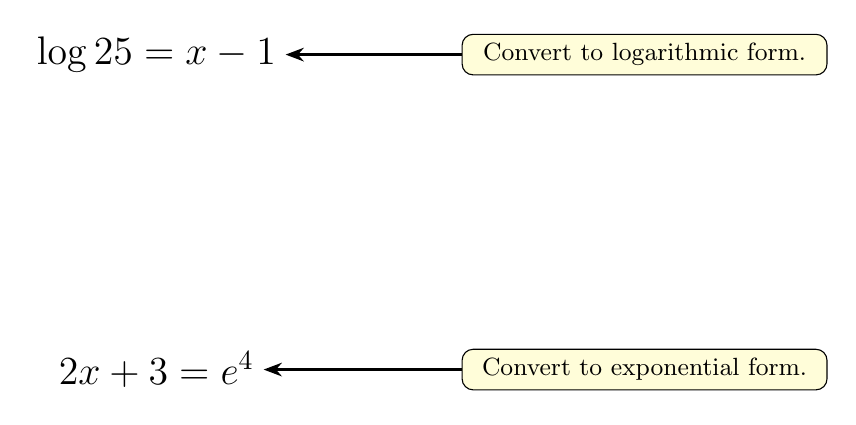
\begin{tikzpicture}[font=\sffamily]
  % Step A: convert to logarithmic form
  \node[font=\Large] (a1) at (0,4) {$\log 25 = x - 1$};
  \node[draw, rounded corners=4pt, fill=yellow!15, text width=4.4cm, align=center,
        font=\small] (c1) at (6.2,4) {Convert to logarithmic form.};
  \draw[-Stealth, thick] (c1.west) to[out=180,in=0] (a1.east);

  % Step B: convert to exponential form
  \node[font=\Large] (a2) at (0,0) {$2x + 3 = e^4$};
  \node[draw, rounded corners=4pt, fill=yellow!15, text width=4.4cm, align=center,
        font=\small] (c2) at (6.2,0) {Convert to exponential form.};
  \draw[-Stealth, thick] (c2.west) to[out=180,in=0] (a2.east);
\end{tikzpicture}
\end{document}
